\newpage
\chapter{Index}\textit{Dennis.}\\
In this chapter an explanation of the index page (front page)  and the different thoughts and actions done with it will be described.  
\section{Design Ideas}
The website is primarily to be used by a non-technical person at AU-Herning. The design has been kept clean to make it very intuitive how to navigate around. Periodically the energy system (and thereby also the website) is shown for high-school students visiting the school, therefore the index page has been build up with mostly icons instead of text and a navigation bar which some of them might know from Apples operation system OS X. The customer wanted the production shown as primitive things like: lightbulbs, refrigerators, money (possibly shown as number of SU payments), instead of technical terms like Joule, kW, kWh etc.
\begin{figure}[h!]
	\center
		\setlength\fboxsep{0pt}
		\setlength\fboxrule{1pt}
		\fbox{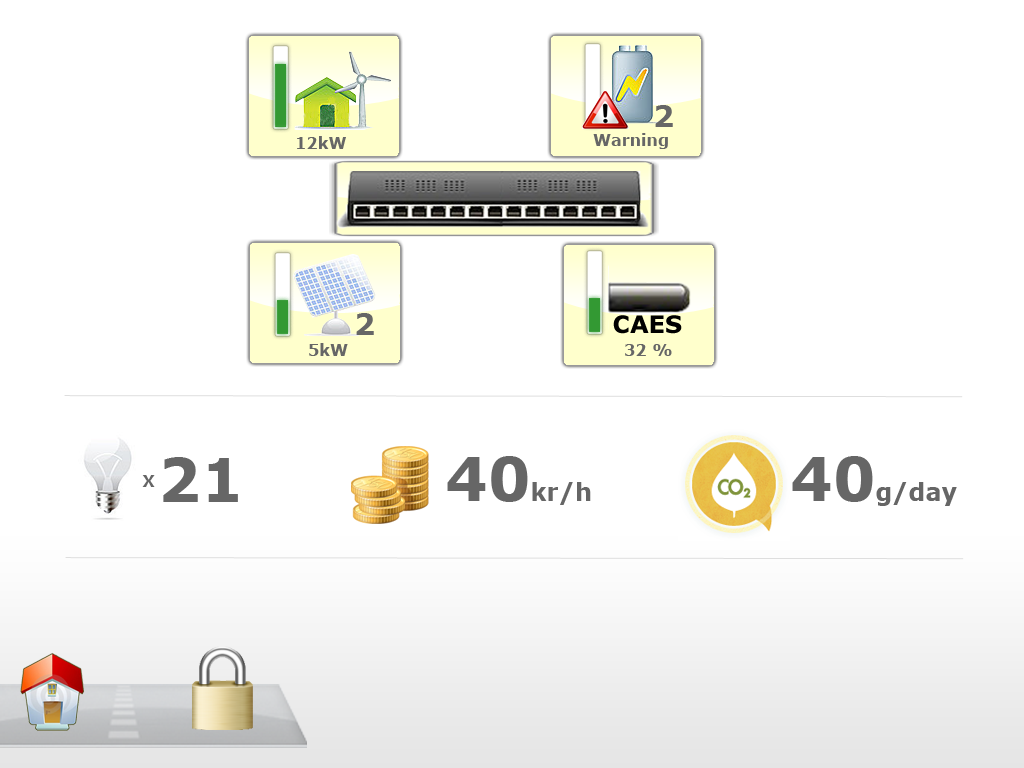
\includegraphics[width=0.5\textwidth]{images/index_design.png}}
   	\caption{Photoshop, final drawings of the index page.}
   	\label{fig:index_page_design}
\end{figure}
\section{The Design}

\begin{figure}[h!]
	\center
		\setlength\fboxsep{0pt}
		\setlength\fboxrule{1pt}
		\fbox{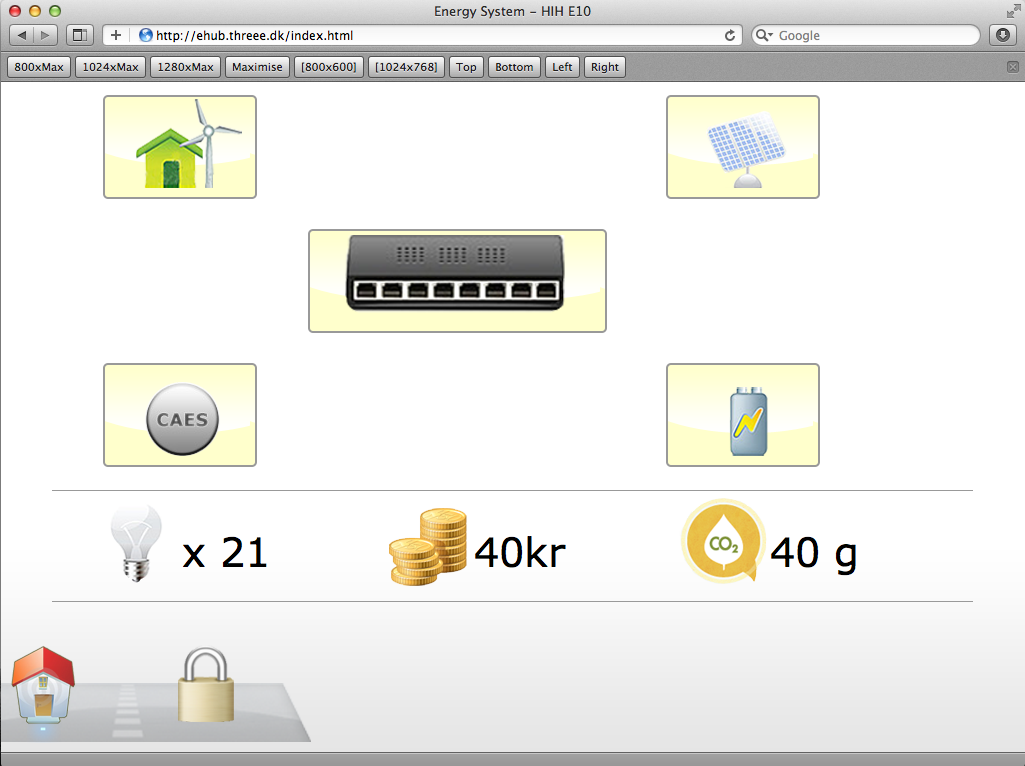
\includegraphics[width=0.6\textwidth]{images/screen_index_page.png}}
   	\caption{The final index page as seen on the website.}
   	\label{fig:index_page_design}
\end{figure}
The background is chosen to be white/grey to keep it simple and not steal focus from the content of the page, but also a clean color seemed to boring and unprofessional. 
\newpage The page is divided into 3 sections:
\begin{itemize}
	\item Modules connected.
	\item Production (shown in an alternative way).
	\item Menu dock.
\end{itemize}
Apples operation system has inspired to the creation of the dock, which is rather different than most other webpages, where the menu bar is normally placed in the top-center or in the left side. The production is shown in non-technical terms to make it more interesting for high-school students or similar, than terms like kW, kWh, Joules. In the top is shown the different modules connected which also works as links to the modules page, where a detailed description of the module can be found. Energy bars, amount of connected modules and status of them will be implemented using Javascript, but so far the page only works as a dummy one, where the style of it can be seen an the way of jumping between between pages works.  
\section{Code layout}
As the site shall be written in strict XHTML, the HTML files will only contain all div's, text and it is also here it is specified which things that should work as links. The style sheet then contains everything else, sizes and positions of divs, pictures, text etc.
\\Doctype and meta tags are described in the next chapter.
\section{Code explanation}
The coding of the index page is explained here. Pieces of the HTML and CSS code is inserted and explained.
\subsection{General setup}
All text needs to be setup as the reset.css file is included. The font family and the h1 tag is the only ones used on the index page. 
\begin{lstlisting}[language=CSS]
body {
	font-family:Verdana, Geneva, sans-serif;
}
h1 { font-size: 40px; }
\end{lstlisting}

\subsection{Background image}
As the background is not proper for repeating in the y direction, it is instead stretched to fit the whole screen. As a background image cannot be stretched in the CSS file, the picture is instead added in the HTML file, in an 'empty div' (as this div only contains the background picture).
\begin{lstlisting}
<div id="bg">
		<img src="pic/background.png" alt="background"/>
</div>
\end{lstlisting}
The picture in the background div is stretched by setting the width and the height of it to 100\%. The picture is putted to the background by using z-index. The setup of which elements should be in front of others is setup using z-index, -999 is used to be sure that no elements is behind the background.
\begin{lstlisting}[language=CSS] 
#bg {}	/*Empty ID for the background to satisfy W3 verificator*/
		
#bg img {	/*Stretch the background image over the whole screen*/
  position: absolute;
  width: 100%;
  height: 100%;
  z-index: -999;	/*Put image behind everything else*/
}
\end{lstlisting}

\subsection{Modules connected}
The connected modules all works as links to their module pages. The 'a' tag is used as a link to another page using the href attribute to a relative URL. The item which is used as the link is a picture showing the module. The module is inserted using the 'img' tag. 'src' specifies the URL of the image and the 'alt' attribute defines an alternative text if the picture cannot be found or shown. All other optional attributes is setup in the CSS file to keep the strict HTML coding.
\begin{lstlisting}
<div id="hub" class="boxbg">
		<a href="hub.html"> <img src="pic/hub_big.png" alt="HUB Module"/> 	</a>
</div>
<div id="Mtopleft" class="boxbg">
		<a href="wind.html"> <img src="pic/wind.png" alt="HUB Module"/> 		</a>
</div>
...
\end{lstlisting}
The position of the 5 modules (4 plus the hub) is set according to percentage of the browser to make use of the whole browser window. Each div has both a class, where general things for the 5 modules are defines, and an id defining the position of each module. The class of the modules sets the background of the modules and repeats it in the x direction. A border around the module divs is also defined with line size 2px and a grey color. The corners of the box is rounded, this does however not work in IE versions older than 9.
\begin{lstlisting}[language=CSS]
.boxbg {
	position:absolute;
	background-image:url(pic/ybg.png);
	background-repeat:repeat-x;
	height: 100px;
	width: 150px;
	border: 2px solid #999;	/* Put padding and round corners*/
	border-bottom-left-radius: 5px;
	border-bottom-right-radius: 5px;
	border-top-left-radius: 5px;
	border-top-right-radius: 5px;
}
	/*Center img*/
.boxbg img { padding-left: 10%; }
	/*HUB position and size*/
#hub {left: 30%; top: 22%; width:295px;}
	/*Module Top left position*/
#Mtopleft {left: 10%; top: 2%;}
...
\end{lstlisting}

\subsection{Energy readout}
The middle section with alternative energy readout has a big div surrounding 3 divs each containing a picture and some text.
\begin{lstlisting}
<div id="linebox">
		<div class="energyboxes" id="bulb">
				<h1>x 21</h1>
		</div>
		...
</div>
\end{lstlisting}
The top and bottom border of the big div is drawn, to make a section split between the modules, energy readout and the dock. A thing to notice is the use of position inherit instead of position absolute. Where position absolute takes the position from the corners of the browser, position inherit positions according to the div it is placed inside. As the energyboxes is placed inside the big div with id linebox, the top and bottom command will position according to the 'linebox' div. Again a class is made to setup general things for the 3 energy divs, and 1 id for each of them to position then and in this case to also insert a different background image to all of them. The idea is that the pictures of the alternative energy should be shown all the time, whereas the modules should only be shown if they are connected and that is why they are inserted in the HTML code.
\begin{lstlisting}[language=CSS]
#linebox {
	position: absolute;
	top: 61%;
	left: 5%;
	width:90%;
	height:110px;
	border-bottom: 1px solid #999;
	border-top: 1px solid #999;
}
.energyboxes {
	position:inherit;
	height: 70px;
	width: 200px;
	background-repeat:no-repeat;
	background-position:left;
	text-align:right;
	padding-top:30px;
}
	/*Position and picture of the bulb div*/
#bulb { left: 2%; background-image:url(pic/bulb.png);}
...
\end{lstlisting}

\subsection{Dock}
On the index page the dock contains only two items, the home button and a locker. At the time the locker links to the index page, but when Javacode is created, it will show an open locker when the user is logged in. Note here that the locker uses a special id, which is defined in the CSS file. The dot under the house shows the current position on the site. It is not used for anything specific on the index page but only there too keep the clean design. On the module pages it is shown under the selected device.
\begin{lstlisting}
<div id="dock">
		<a href="index.html"> <img src="pic/dock_home.png" 		alt="home" /> 					</a>
		<a href="index.html"> <img src="pic/dock_key_lock.png" 	alt="key_locked"  id="lock" /> 	</a>
</div>
<div id="dot">
		<img src="pic/dot.png" alt="dot" />
</div>
\end{lstlisting}
Opposite the background which was z-index'ed -999, the dot is indexed to 1 to bring it in front of everything else. In line 13 is defined a special id for the locker picture, the picture is set to position according to the right side of the div it is placed in. All links in the dock are slightly see through to create some simple graphic changes when the user holds the mouse over the icons. At mouse over the opacity is removed. The mouse over is done by using the img:hover command, where the img says that it is an image that the mouse can be held over.
\begin{lstlisting}[language=CSS]
#dock {
	position: absolute;
	width: 310px;
	background-image:url(pic/dock_small.png);
	background-repeat: no-repeat;
	background-position: bottom;
	bottom: 10px;
	height: 100px;
}
#dock img {float: left; opacity:0.80;} /*All browsers exept IE*/

	/*change position of the locker to float right instead of left as the other link(s)*/
img#lock { float: right; padding-right: 50px;}
	/*remove transparency when mouse over*/
#dock img:hover {opacity:1.00;}  /*All browsers exept IE*/
	/*set dot position to under the house (home)*/
#dot {
	position: absolute;
	bottom: 3px;
	left: 26px;
	z-index: 1; /*put in front of everything else*/
}
\end{lstlisting}
